\LARGE{ \textbf {Лекция №8}}\\
\Large{ \textbf {}}\\
\textbf{Синхронные триггеры с 2-ступеньчатым запоминанем информации и со статическим управлением запиьсю.}\\
MS-тр-р.\\
Имеют 2 ступени запоминания информации . 1 - основной триггер. 2 - вспомогательный триггер.\\
Принцип действия:\\
При с = 1 разрешена запись входной инфы в первую ступень и запрещена передача во вторую ступень.
По окончании действия синхросигнала(с = 0) информация из первой ступени переписывается во вторую ступень.\\
Управляющая связь между основным и вспомогательными триггерами может осуществляться следующими способами:

\begin{enumerate}
  \item С инвертором синхросигнала.
  \item С запрещающими связями.
  \item С разнополярным управлением.
  \item С коммутирующими транзисторами.
\end{enumerate}

\Large{Двуступеньчатый синхронный RS триггер с запрещающим инвертором. }\\
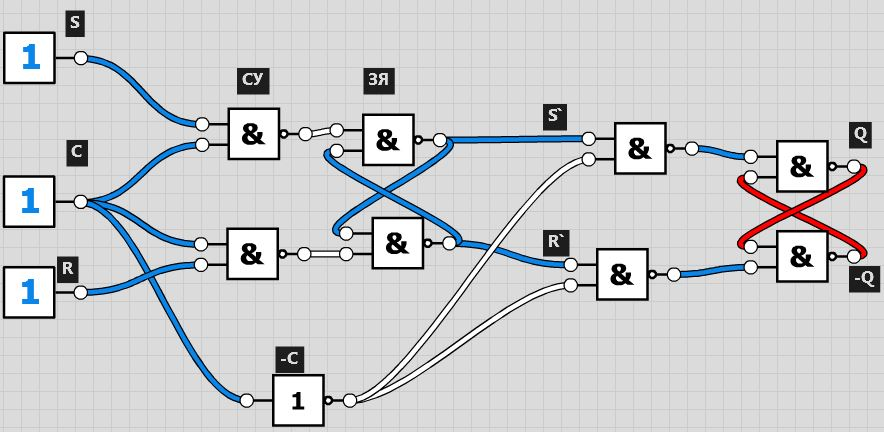
\includegraphics[width=\linewidth*3/4]{27} \\

% \Large{Двуступеньчатый асинхронный RS триггер с запрещающим инвертором. }\\
% 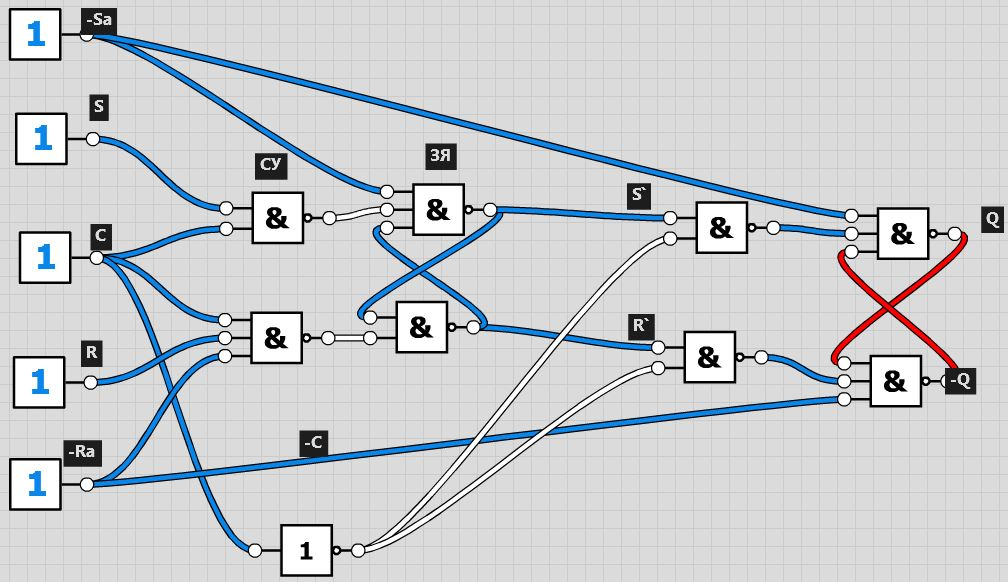
\includegraphics[width=\linewidth*3/4]{28} \\

Принцип функционирования ЖК триггера почти такой же как и RS.\\
J 0 0 1 1 \\
K 0 1 0 1 \\
хранение, установка в 0,установка в 1, переключение в противположное состояние. \\
$t_{impls} => 3t^*_{zaderSR}$\\
$t_{pause} => 3t^*_{zaderSR} + t^{NE}_{zaderSR} $\\
$t_{pause} => 4t^*_{zaderSR} $\\
$T^{triger}=>t_{impls} + t_{pause}  => 7 t^*_{zaderSR}$ \\

Для ЖК триггера может использоваться только эта схема.\\


Синхронные двуступеньчатые триггеры с запрещающими связями.\\
Синхронный двуступеньчатый ЖК-триггер.\\

При с = 1 и любых сочетаниях сигналов J и K , кроме J=K=0. В состоянии 0 окажется лог. элемент 1 либо лог. элемент 2.
0 с выходовох этих элементов попадают на входы эл 5 и 6 и запрещают запись информации во вторую ступень.\\
При с =0 разрешен прием информации во вторую ступень.\\
При этом Sa = Ra = 1 \\
Реализация двухступенчатого JK-триггера на базе элементов "И-НЕ".\\
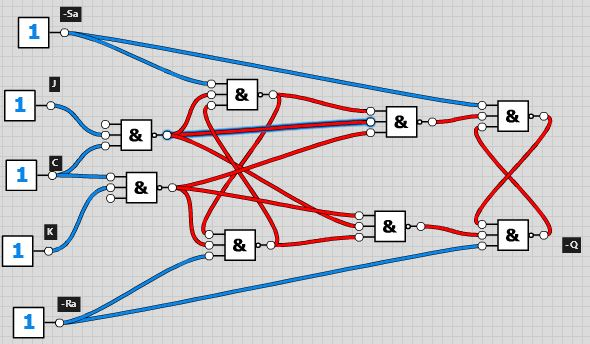
\includegraphics[width=\linewidth]{20}
